\section{Experiments}

\begin{table*}[t]
  \caption{\textbf{Main results.} Accuracy (\%) on AI2-THOR (in-domain) and different-environment (out-of-domain) benchmarks. PT reports the average across input settings (EgoDir/Path/PathArr for AI2-THOR; Real/Real+Arr for different environments). Text CoT generates a textual chain-of-thought before answering. IPT (Imaginative Perception Token) generates an intermediate image before answering. For our models, accuracy reports the \textbf{maximum} between answer-only and free-generation inference. Best per group in \textbf{bold}.}
  \vspace{-1em}
  \centering
  \setlength{\tabcolsep}{13pt}
  % \resizebox{\columnwidth}{!}{
  \begin{tabular}{l ccc cc}
    \toprule
    & \multicolumn{3}{c}{\textbf{AI2-THOR}} & \multicolumn{2}{c}{\textbf{Different Env.}} \\
    \cmidrule(lr){2-4} \cmidrule(lr){5-6}
    \textbf{Model}
      & PET & \footnotesize PT & MVC
      & \footnotesize PET & \footnotesize PT \\
    \midrule
    \multicolumn{6}{l}{\emph{VQA Models}} \\
    GPT-5            & \textbf{79.8} & \textbf{60.2} & 53.5 & \textbf{69.3} & \textbf{80.9} \\
    GPT-5.2          & 45.5 & 32.9 & 44.2 & 54.0 & 63.0 \\
    Gemini 2.5 Flash & 51.0 & 41.5 & 30.8 & 66.3 & 71.4 \\
    Gemini 3 Flash   & 55.0 & 42.3 & \textbf{56.9} & 51.3 & 83.2 \\
    InternVL3.5-8B   & 51.5 & 35.8 & 44.6 & 47.7 & 47.4 \\
    Qwen2.5-VL-7B   & 50.7 & 37.3 & 38.8 & 54.3 & 44.8 \\
    Qwen3-VL-8B     & 52.0 & 35.9 & 43.8 & 46.7 & 64.1 \\
    \midrule
    \multicolumn{6}{l}{\emph{Unified Models}} \\
    Janus-Pro-7B     & 51.8 & 33.5 & 33.1 & 44.7 & 35.3 \\
    Chameleon 7B     & 34.3 & 16.3 & 5.4 & 47.3 & 24.5 \\
    \midrule
    \multicolumn{6}{l}{\emph{Ours (fine-tuned BAGEL)}} \\
    Bagel (base)              & 40.3 & 29.9 & 35.4 & 62.7 & 42.7 \\
    Bagel (label-only)        & 97.5 & 65.7 & 63.9 & 82.0 & 54.7 \\
    + Text CoT                 & 83.1 & 49.7 & 62.3 & 70.3 & 52.2 \\
    + IPT                       & 96.8 & 49.0 & \textbf{67.3} & 87.0 & 57.5 \\
    + Mixed Training            & \textbf{97.8} & \textbf{66.7} & 62.3 & \textbf{87.7} & \textbf{58.6} \\
    \bottomrule
  \end{tabular}
  % }
  \label{tab:main_results}
\end{table*}


We evaluate \emph{imaginative perception tokens} on the three spatial reasoning tasks introduced in \cref{sec:data}: \textbf{Perspective Taking (PET)}, \textbf{Path Tracing (PT)}, and \textbf{Multiview Counting (MVC)}. To enable controlled comparisons, we train all task-specific models on the AI2-THOR subset of each dataset. We additionally report transfer to cross-environment benchmarks (Habitat), real-world images, and external datasets. All tasks use multiple-choice evaluation with balanced answer distributions.

PT is evaluated under three input variants that provide increasing spatial cues: \textbf{EgoDir} (egocentric direction only), \textbf{Path} (top-down path overlay), and \textbf{PathArr} (path with directional arrows) and average accuracy reported. Unless otherwise stated, we report accuracy (\%) and use the same prompt formatting across baselines and our models.

\subsection{Setup}

\noindent\textbf{Baselines.}
We compare against two groups of models, evaluated zero-shot with task-specific prompts.
\emph{VQA models} include GPT-5, GPT-5.2, Gemini~2.5 Flash, Gemini~3 Flash, InternVL3.5-8B, Qwen2.5-VL-7B, and Qwen3-VL-8B.
\emph{Unified models} that support both understanding and generation include Janus-Pro-7B and Chameleon~7B.

\noindent\textbf{Our model variants.}
We fine-tune BAGEL~\cite{deng2025bagel} under several configurations to isolate the contribution of imagination supervision. Each fine-tuned model is task-specific and trained on a single task using AI2-THOR data only (unless noted otherwise):
\begin{itemize}
    \item \textbf{Bagel (base)}: pretrained model with no task-specific fine-tuning.
    \item \textbf{Bagel (label-only)}: fine-tuned with answer supervision only, with no intermediate thought.
    \item \textbf{+ Text CoT}: trained to generate a textual chain-of-thought describing the imagined spatial configuration before answering. Training CoTs are generated by GPT-5.1 using simulator ground-truth scene metadata.
    \item \textbf{+ IPT}: trained to generate an intermediate image (the imaginative perception token) before answering.
    \item \textbf{+ Mixed Training}: trained on a mixture of IPT examples (image-generation targets) and label-only examples (answer supervision only).
\end{itemize}

\noindent\textbf{Training details.}
We fine-tune BAGEL-7B-MoT with AdamW (lr $1{\times}10^{-5}$, $2{,}000$ warmup steps) on $8$ GPUs using FSDP bf16, following BAGEL~\cite{deng2025bagel} and ThinkMorph~\cite{gu2025thinkmorph}.
For multi-image inputs, each image is resized to $512{\times}512$.
Unless noted, IPTs use Latent-64 resolution.
\vspace{-0.5em}
\subsection{Main results}

Table~\ref{tab:main_results} reports results on our benchmarks.

\begin{takeawayblock}
    \textbf{Spatial reasoning remains difficult for current VLM and unified models.}
\end{takeawayblock}
Among the zero-shot baselines, GPT-5 is the strongest across nearly all settings, yet still trails our best fine-tuned variants on multiple in-distribution tasks.
Smaller open VLM models (InternVL3.5-8B, Qwen2.5-VL-7B, Qwen3-VL-8B) hover near chance on PET (50--52\%) and struggle on PT, indicating that these tasks are not solvable through superficial cues.
Unified models perform worse overall: Chameleon~7B drops to 34.3\% on PET and 5.4\% on MVC, suggesting that current unified designs often trade away understanding robustness in exchange for generation capability.

\begin{takeawayblock}
    \textbf{Answer supervision alone yields large gains and transfers across environments.}
\end{takeawayblock}
Bagel (label-only) substantially improves over Bagel (base) across all tasks, rising from 40.3\% to 97.5\% on AI2-THOR PET, from 29.9\% to 65.7\% on PT, and from 35.4\% to 63.9\% on MVC.
These improvements transfer: label-only reaches 82.0\% on Habitat PET, showing that spatial reasoning can be learned in simulation and generalized to new environments.

\begin{takeawayblock}
    \textbf{Imagination supervision helps most when language is a poor interface.}
\end{takeawayblock}
On MVC, IPT achieves the best accuracy (67.3\%), outperforming label-only (63.9\%) and Text CoT (62.3\%).
On different-environment PET (Habitat), IPT reaches 87.0\% (vs.\ 82.0\% for label-only), and Mixed Training improves further to 87.7\%.
On PT, Mixed Training achieves the best results on both synthetic (66.7\%) and real (58.6\%) benchmarks, outperforming label-only (65.7\% / 54.7\%) and all baselines.
IPT also improves real-world PT transfer (57.5\%) over label-only (54.7\%) and Text CoT (52.2\%).
Notably, IPT models are evaluated in \emph{answer-only} mode: the model does not generate an image at inference, yet the imagination targets during training strengthen internal spatial representations that transfer across environments.

\begin{takeawayblock}
    \textbf{Text CoT underperforms label-only and IPT.}
\end{takeawayblock}
Text CoT typically falls behind label-only (e.g., PET 83.1\% vs.\ 97.5\%, PT 49.7\% vs.\ 65.7\%) and also behind IPT (e.g., MVC 62.3\% vs.\ 67.3\%, PET 83.1\% vs.\ 96.8\%).
Compared to label-only, the Text CoT objective forces the model to allocate capacity to generating long spatial descriptions during fine-tuning, which competes with answer prediction.
Compared to IPT, the gap reflects a modality mismatch: viewpoint changes, occlusions, and cross-view correspondences are difficult to serialize into natural language, and the resulting textual traces introduce noise rather than useful structure. IPT represents these relationships directly in the visual modality where they are naturally expressed.
\vspace{-1em}
\subsection{Ablations}
\label{sec:exp_ablation}

\begin{figure*}[t]
  \centering
  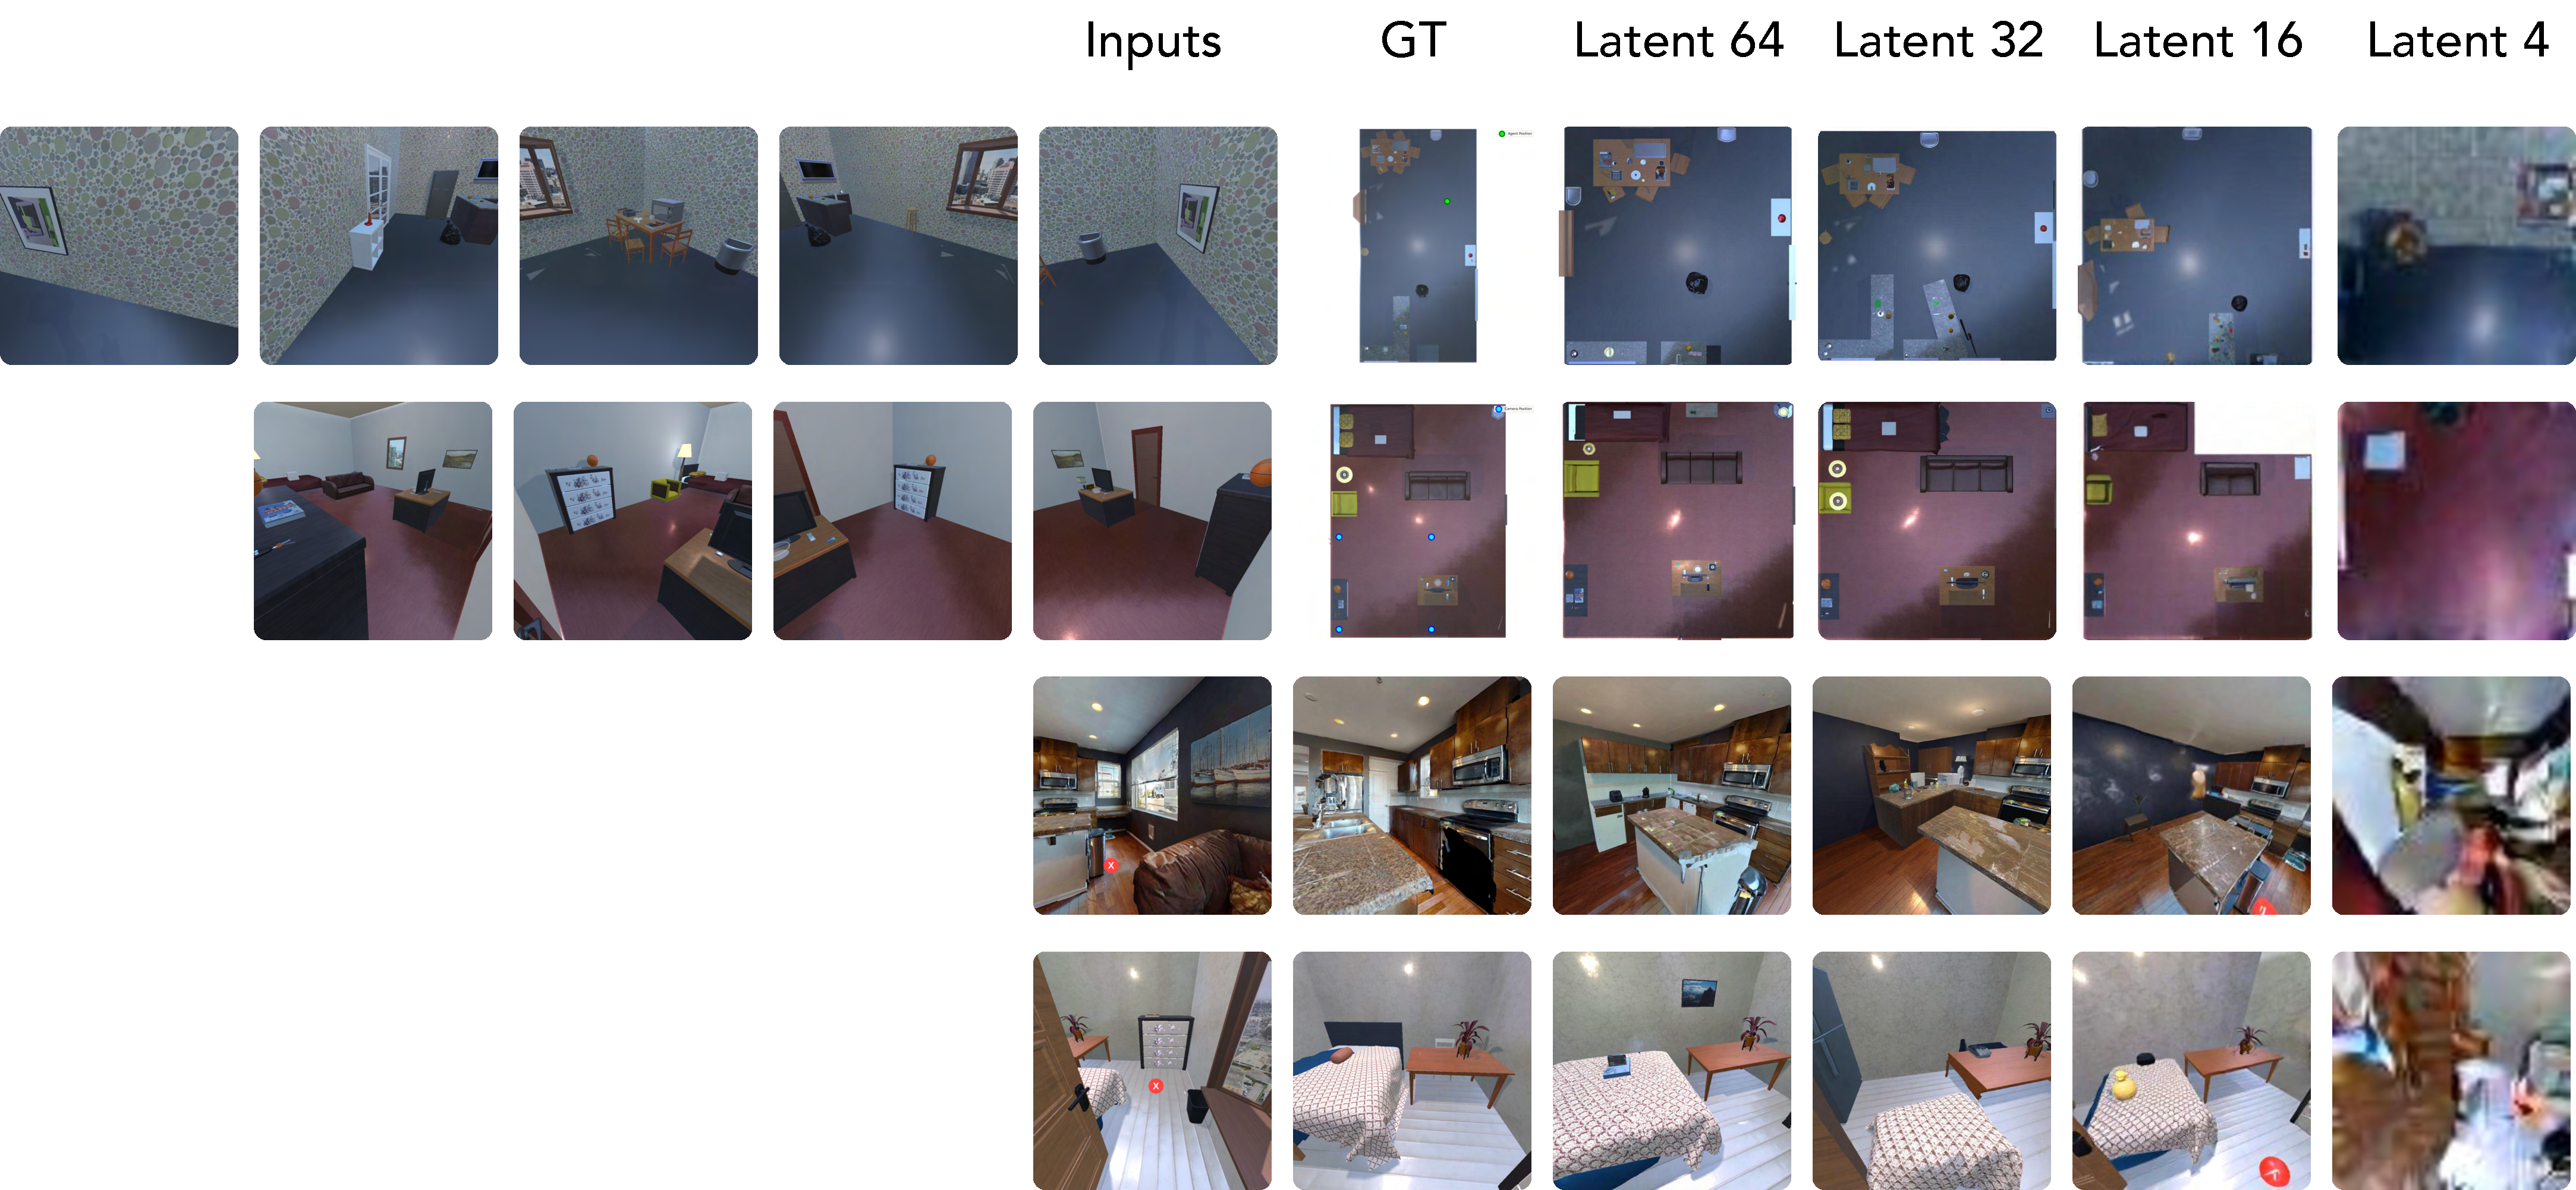
\includegraphics[ height=0.3\linewidth]{imgs/latent.pdf}
  \caption{Qualitative examples of model-generated imaginative perception tokens. Top two rows: MVC example showing imagined top-down BEV maps. Bottom: PET examples showing imagined novel viewpoints. From left to right, imagination resolution increases from Latent-4 ($64\times 64$) to Latent-64 ($1024\times 1024$). Higher resolution produces sharper and more spatially faithful imaginations, preserving object identities and relative positions needed for downstream reasoning.}
  \label{fig:ablation_latent}
\end{figure*}
% \FloatBarrier
\begin{table}[t]
  \caption{\textbf{Ablation on latent size.} Accuracy (\%) with w/ Thought inference mode at different imagination resolutions. Best per column in \textbf{bold}.}
  \vspace{-1em}
  \centering
  \setlength{\tabcolsep}{6pt}
  \small
  \begin{tabular}{l c cc c}
    \toprule
    & & \multicolumn{2}{c}{\textbf{PET}} & \textbf{MVC} \\
    \cmidrule(lr){3-4} \cmidrule(lr){5-5}
    \textbf{Latent Size} & \textbf{Resolution}
      & \footnotesize AI2-THOR & \footnotesize Habitat
      & \footnotesize AI2-THOR \\
    \midrule
    Latent-4  & $64\times64$     & 87.4 & 73.3 & 53.5 \\
    Latent-16 & $256\times256$   & 95.3 & 81.0 & 56.2 \\
    Latent-32 & $512\times512$   & 95.0 & \textbf{87.0} & 58.9 \\
    Latent-64 & $1024\times1024$ & \textbf{96.8} & 83.3 & \textbf{63.1} \\
    \bottomrule
  \end{tabular}
  \label{tab:ablation_latent}
\end{table}

\begin{takeawayblock}
    \textbf{Latent resolution controls imagination quality and downstream accuracy.}
\end{takeawayblock}
\Cref{tab:ablation_latent,fig:ablation_latent} ablate IPT resolution on PET and MVC.
At Latent-4 ($64\times64$), imaginations are blurry and lose spatial detail; at Latent-64 ($1024\times1024$), imaginations become sharper and more spatially faithful, preserving object identities and relative positions.
Quantitatively, increasing resolution from Latent-4 to Latent-64 improves AI2-THOR PET from 87.4\% to 96.8\% and MVC from 53.5\% to 63.1\%.
Habitat PET peaks at Latent-32 (87.0\%) and drops slightly at Latent-64 (83.3\%), suggesting mild overfitting to AI2-THOR appearance statistics at the highest resolution.

\begin{table}[t]
  \caption{\textbf{Ablation on thought modality and inference mode.} Accuracy (\%) on AI2-THOR benchmarks (PT uses EgoDir variant). We compare Text CoT vs.\ IPT training and vary inference mode: generate thought then answer (w/ text/image), answer directly (answer-only), or condition on ground-truth (w/ GT image).}
  \vspace{-1em}
  \centering
  \setlength{\tabcolsep}{6pt}
  \small
  \begin{tabular}{ll ccc}
    \toprule
    \textbf{Training} & \textbf{Inference} & \textbf{PET} & \textbf{PT} & \textbf{MVC} \\
    \midrule
    Text CoT   & w/ text      & 83.1 & 53.1 & 61.5 \\
    Text CoT   & answer-only  & 78.3 & 55.8 & 62.3 \\
    \midrule
    IPT        & w/ image     & 96.8 & 50.4 & 63.1 \\
    IPT        & answer-only  & 96.8 & 61.1 & 62.3 \\
    \midrule
    IPT        & w/ GT image  & 96.7 & \textbf{86.7} & \textbf{67.3} \\
    \bottomrule
  \end{tabular}
  \label{tab:ablation_thought}
\end{table}
\vspace{-1em}
\paragraph{Thought modality and inference mode.}
Table~\ref{tab:ablation_thought} ablates the training signal (Text CoT vs.\ IPT) and inference mode (generate thought, answer-only, or oracle GT).

\begin{takeawayblock}
    \textbf{IPT training builds stronger spatial representations than Text CoT.}
\end{takeawayblock}
On PT, IPT with answer-only inference (61.1\%) outperforms Text CoT with answer-only inference (55.8\%) by 5.3 points.
On MVC, IPT with image generation (63.1\%) outperforms Text CoT with text generation (61.5\%).

\begin{takeawayblock}
    \textbf{Imagination supervision is useful, but explicit generation is not required at inference.}
\end{takeawayblock}
For IPT models, answer-only mostly outperforms generating the imagination explicitly: on PT, answer-only reaches 61.1\% vs.\ 50.4\% with generation.
For Text CoT, generating the chain-of-thought also slightly underperforms answer-only (53.1\% vs.\ 55.8\% on PT), though the gap is smaller than for IPT.
This asymmetry suggests that producing faithful imaginations is harder than producing text descriptions, and imperfect generations can mislead downstream reasoning. However, training with imagination targets remains valuable: answer-only IPT matches GPT-5 on PT (61.1\%).

\begin{takeawayblock}
    \textbf{Ground-truth imaginations reveal headroom.}
\end{takeawayblock}
When given ground-truth imaginations instead of model-generated ones, PT accuracy jumps from 50.4\% to 86.7\% (+36.3) and MVC rises from 63.1\% to 67.3\% (+4.2).
The large PT gap indicates that imagination quality is the dominant bottleneck for path tracing; for PET, model-generated imaginations nearly match GT (96.8\% vs.\ 96.7\%), leaving little room for improvement.

\begin{table}[t]
  \caption{\textbf{Transfer to similar external benchmarks.} Accuracy (\%). SAT tests perspective taking and MessyTable tests multiview counting, both in domains unseen during training. Best in \textbf{bold}.}
  \vspace{-1em}
  \centering
  \setlength{\tabcolsep}{6pt}
  \small
  \begin{tabular}{l cc}
    \toprule
    & \textbf{PET} & \textbf{MVC} \\
    \cmidrule(lr){2-2} \cmidrule(lr){3-3}
    \textbf{Model}
      & \footnotesize SAT (66)
      & \footnotesize MessyTable (200) \\
    \midrule
    Bagel (base)       & 34.9 & 29.0 \\
    Bagel (label-only) & 59.1 & 32.5 \\
    + Text CoT         & 50.0 & 30.0 \\
    + IPT              & 57.6 & 28.5 \\
    + Mixed Training   & \textbf{63.6} & \textbf{37.0} \\
    \bottomrule
  \end{tabular}
  \label{tab:transfer}
\end{table}
\vspace{-1em}


\begin{takeawayblock}
    \textbf{IPT transfers to aligned external benchmarks.}
\end{takeawayblock}
Table~\ref{tab:transfer} evaluates transfer to external benchmarks that test similar spatial capabilities: SAT~\cite{ray2025satdynamicspatialaptitude} (perspective-taking subset) and MessyTable~\cite{cai2020messytable} (multiview counting).
On SAT, Bagel (label-only) improves from 34.9\% to 59.1\% over Bagel (base), and Mixed Training further improves to 63.6\%.
On MessyTable, Mixed Training reaches 37.0\%, up from 29.0\% for Bagel (base).

\begin{table}[t]
  \caption{\textbf{Does our data help on other spatial tasks?} Accuracy (\%) on benchmarks beyond our training task categories. Fine-tuning on our AI2-THOR MVC data consistently improves over Bagel (base), suggesting that the spatial reasoning learned from our datasets transfers broadly. Best per column in \textbf{bold}.}
  \vspace{-1em}
  \centering
  \setlength{\tabcolsep}{4pt}
  \small
  \begin{tabular}{l ccc}
    \toprule
    \textbf{Model}
      & \footnotesize ScanNet (200)
      & \footnotesize MindCube (200)
      & \footnotesize All-Angles (170) \\
    \midrule
    \multicolumn{4}{l}{\emph{VQA Models}} \\
    GPT-5            & 58.5 & \textbf{67.3} & \textbf{67.9} \\
    GPT-5.2          & 48.5 & 37.5 & 29.4 \\
    Gemini 2.5 Flash & 48.0 & 50.3 & 37.9 \\
    Gemini 3 Flash   & 62.5 & 56.5 & 64.2 \\
    InternVL3.5-8B   & 53.5 & 42.1 & 54.8 \\
    Qwen2.5-VL-7B   & \textbf{63.5} & 47.8 & 51.8 \\
    Qwen3-VL-8B     & 62.5 & 34.5 & 42.3 \\
    \midrule
    \multicolumn{4}{l}{\emph{Unified Models}} \\
    Janus-Pro-7B     & 39.5 & 42.0 & 45.0 \\
    Chameleon 7B     & 5.5 & 25.4 & 17.7 \\
    \midrule
    \multicolumn{4}{l}{\emph{Ours (fine-tuned BAGEL)}} \\
    Bagel (base)       & 40.5 & 39.5 & 40.0 \\
    Bagel (fine-tuned) & \textbf{52.0} & \textbf{47.5} & \textbf{50.0} \\
    \bottomrule
  \end{tabular}
  \label{tab:ablation_data}
\end{table}


\begin{takeawayblock}
    \textbf{Training with our data improves performance on other spatial benchmarks.}
\end{takeawayblock}
Finally, we test whether our training data improves spatial reasoning on tasks with different structures: ScanNet~\cite{dai2017scannet} (in-the-wild multiview counting), MindCube~\cite{yin2025mindcube} (abstract geometric reasoning), and All-Angles-Bench~\cite{yeh2025seeing} (cross-view matching on EgoHumans~\cite{khirodkar2023egohumans}).
Because IPTs are task-specific by construction (e.g., rotated views for PET, bird's-eye paths for PT), they do not directly transfer to these settings. We therefore fine-tune on AI2-THOR MVC using answer supervision only.
Bagel (fine-tuned) consistently improves over Bagel (base) across all three benchmarks (40.5\%$\to$52.0\% on ScanNet, 39.5\%$\to$47.5\% on MindCube, 40.0\%$\to$50.0\% on All-Angles), indicating that our simulator data builds broadly useful spatial representations even when the specific imaginative token target changes.
